\documentclass[12pt,preprint, authoryear]{elsarticle}

\usepackage{lmodern}
%%%% My spacing
\usepackage{setspace}
\setstretch{2}
\DeclareMathSizes{12}{14}{10}{10}

% Wrap around which gives all figures included the [H] command, or places it "here". This can be tedious to code in Rmarkdown.
\usepackage{float}
\let\origfigure\figure
\let\endorigfigure\endfigure
\renewenvironment{figure}[1][2] {
    \expandafter\origfigure\expandafter[H]
} {
    \endorigfigure
}

\let\origtable\table
\let\endorigtable\endtable
\renewenvironment{table}[1][2] {
    \expandafter\origtable\expandafter[H]
} {
    \endorigtable
}


\usepackage{ifxetex,ifluatex}
\usepackage{fixltx2e} % provides \textsubscript
\ifnum 0\ifxetex 1\fi\ifluatex 1\fi=0 % if pdftex
  \usepackage[T1]{fontenc}
  \usepackage[utf8]{inputenc}
\else % if luatex or xelatex
  \ifxetex
    \usepackage{mathspec}
    \usepackage{xltxtra,xunicode}
  \else
    \usepackage{fontspec}
  \fi
  \defaultfontfeatures{Mapping=tex-text,Scale=MatchLowercase}
  \newcommand{\euro}{€}
\fi

\usepackage{amssymb, amsmath, amsthm, amsfonts}

\def\bibsection{\section*{References}} %%% Make "References" appear before bibliography


\usepackage[round]{natbib}

\usepackage{longtable}
\usepackage[margin=2.3cm,bottom=2cm,top=2.5cm, includefoot]{geometry}
\usepackage{fancyhdr}
\usepackage[bottom, hang, flushmargin]{footmisc}
\usepackage{graphicx}
\numberwithin{equation}{section}
\numberwithin{figure}{section}
\numberwithin{table}{section}
\setlength{\parindent}{0cm}
\setlength{\parskip}{1.3ex plus 0.5ex minus 0.3ex}
\usepackage{textcomp}
\renewcommand{\headrulewidth}{0.2pt}
\renewcommand{\footrulewidth}{0.3pt}

\usepackage{array}
\newcolumntype{x}[1]{>{\centering\arraybackslash\hspace{0pt}}p{#1}}

%%%%  Remove the "preprint submitted to" part. Don't worry about this either, it just looks better without it:
\makeatletter
\def\ps@pprintTitle{%
  \let\@oddhead\@empty
  \let\@evenhead\@empty
  \let\@oddfoot\@empty
  \let\@evenfoot\@oddfoot
}
\makeatother

 \def\tightlist{} % This allows for subbullets!

\usepackage{hyperref}
\hypersetup{breaklinks=true,
            bookmarks=true,
            colorlinks=true,
            citecolor=blue,
            urlcolor=blue,
            linkcolor=blue,
            pdfborder={0 0 0}}


% The following packages allow huxtable to work:
\usepackage{siunitx}
\usepackage{multirow}
\usepackage{hhline}
\usepackage{calc}
\usepackage{tabularx}
\usepackage{booktabs}
\usepackage{caption}


\newenvironment{columns}[1][]{}{}

\newenvironment{column}[1]{\begin{minipage}{#1}\ignorespaces}{%
\end{minipage}
\ifhmode\unskip\fi
\aftergroup\useignorespacesandallpars}

\def\useignorespacesandallpars#1\ignorespaces\fi{%
#1\fi\ignorespacesandallpars}

\makeatletter
\def\ignorespacesandallpars{%
  \@ifnextchar\par
    {\expandafter\ignorespacesandallpars\@gobble}%
    {}%
}
\makeatother

\newenvironment{CSLReferences}[2]{%
}

\urlstyle{same}  % don't use monospace font for urls
\setlength{\parindent}{0pt}
\setlength{\parskip}{6pt plus 2pt minus 1pt}
\setlength{\emergencystretch}{3em}  % prevent overfull lines
\setcounter{secnumdepth}{5}

%%% Use protect on footnotes to avoid problems with footnotes in titles
\let\rmarkdownfootnote\footnote%
\def\footnote{\protect\rmarkdownfootnote}
\IfFileExists{upquote.sty}{\usepackage{upquote}}{}

%%% Include extra packages specified by user
\usepackage{booktabs}
\usepackage{longtable}
\usepackage{array}
\usepackage{multirow}
\usepackage{wrapfig}
\usepackage{float}
\usepackage{colortbl}
\usepackage{pdflscape}
\usepackage{tabu}
\usepackage{threeparttable}
\usepackage{threeparttablex}
\usepackage[normalem]{ulem}
\usepackage{makecell}
\usepackage{xcolor}

%%% Hard setting column skips for reports - this ensures greater consistency and control over the length settings in the document.
%% page layout
%% paragraphs
\setlength{\baselineskip}{12pt plus 0pt minus 0pt}
\setlength{\parskip}{12pt plus 0pt minus 0pt}
\setlength{\parindent}{0pt plus 0pt minus 0pt}
%% floats
\setlength{\floatsep}{12pt plus 0 pt minus 0pt}
\setlength{\textfloatsep}{20pt plus 0pt minus 0pt}
\setlength{\intextsep}{14pt plus 0pt minus 0pt}
\setlength{\dbltextfloatsep}{20pt plus 0pt minus 0pt}
\setlength{\dblfloatsep}{14pt plus 0pt minus 0pt}
%% maths
\setlength{\abovedisplayskip}{12pt plus 0pt minus 0pt}
\setlength{\belowdisplayskip}{12pt plus 0pt minus 0pt}
%% lists
\setlength{\topsep}{10pt plus 0pt minus 0pt}
\setlength{\partopsep}{3pt plus 0pt minus 0pt}
\setlength{\itemsep}{5pt plus 0pt minus 0pt}
\setlength{\labelsep}{8mm plus 0mm minus 0mm}
\setlength{\parsep}{\the\parskip}
\setlength{\listparindent}{\the\parindent}
%% verbatim
\setlength{\fboxsep}{5pt plus 0pt minus 0pt}



\begin{document}



\begin{frontmatter}  %

\title{Much Ado About Dividends}

% Set to FALSE if wanting to remove title (for submission)




\author[Add1]{Gabriel Rambanapasi}
\ead{gabriel.rams44@gmail.com}





\address[Add1]{Stellenbosch University, Cape Town, South Africa}

\cortext[cor]{Corresponding author: Gabriel Rambanapasi}

\begin{abstract}
\small{
Dividend paying stock are commonly employed to introduce an income
component into equity portfolios, with the promise of achieving higher
total returns while managing lower risk. This study examines globally
traded dividend portfolios constructed using high yield or dividend
growth signals. It is observed that the performance of dividend
portfolios varies across geographies;however, high yield strategies
consistently provide investors with the highest aggregate returns in
advanced economies over time. When index returns are stratified, it
becomes apparent that during periods of low volatility, high yield
strategies outperform dividend growth strategies, and all portfolios
yield higher returns during interest rate hiking cycles than during
cutting cycles. The consistency of returns from these portfolios over
time is found to be poor, with South African strategies showing the
highest level of consistency over the past decade when assessed on a
rolling basis. In evaluating portfolio risk by geography, we note that
advanced markets have historically experienced fewer drawdowns, whilst
emerging markets and South Africa have exhibited seemingly improving
risk measures within the same period.
}
\end{abstract}

\vspace{1cm}





\vspace{0.5cm}

\end{frontmatter}

\setcounter{footnote}{0}



%________________________
% Header and Footers
%%%%%%%%%%%%%%%%%%%%%%%%%%%%%%%%%
\pagestyle{fancy}
\chead{}
\rhead{}
\lfoot{}
\rfoot{\footnotesize Page \thepage}
\lhead{}
%\rfoot{\footnotesize Page \thepage } % "e.g. Page 2"
\cfoot{}

%\setlength\headheight{30pt}
%%%%%%%%%%%%%%%%%%%%%%%%%%%%%%%%%
%________________________

\headsep 35pt % So that header does not go over title




\hypertarget{problem-statement}{%
\section{Problem Statement}\label{problem-statement}}

As summarized by Vanguard (2017) succinctly, ``the focus of high
dividend-yielding equities is often their income potential, but higher
yields do not necessarily translate into higher returns. This is
because, for all companies, whether or not to pay a dividend is a
capital budgeting decision. When a stock goes ex-dividend, its price
falls by the same amount as the dividend payment. Therefore, no wealth
is created through paying a dividend; rather, the payment reduces
retained earnings. This means that share price should decrease
accordingly thus share holders should be worse off. Thus, brings in the
question of why dividend strategies provide for a return signalling cue.
First, there should exists a rationale beyond dividend payment effect on
share price, perhaps in line with theories regarding dividend relevance.
Second, if the signals provide some type excess return beyond their
market index, does it continuously provide the premium to be harvested
by a systematic investment strategy.

\hypertarget{research-aim}{%
\section{Research Aim}\label{research-aim}}

The aim of this study is to test whether and why dividend payout
strategies contain a profitable investment signal to potential
investors. There exists various international studies testing this
hypothesis across geographies, underscoring that dividend can be used as
a profitable future return signal. Studies conducted for the South
African market employ methodologies that do not inform readers on
mechanisms behind why the dividend signal works or provide an indication
of returns for a systematic dividend investment strategy. We aim to fill
this gap by testing various portfolios constructed based on dividend
information in South Africa.

\newpage

\hypertarget{introduction}{%
\section{Introduction}\label{introduction}}

This paper seeks to investigate the return signalling cue of dividend
paying stock. The value of dividends towards shareholders has long been
debated with academics and practitioners providing evidence for their
irrelevance and relevance. Miller \& Modigliani
(\protect\hyperlink{ref-miller}{1961}) proposed the dividend irrelevance
theorem that essentially argues that dividend payments were irrelevant
as this detracted from the shareholder value as wealth is affected by
the income a firm generates, not the way the firm distributes that
income. Against this, Gordon (\protect\hyperlink{ref-gordon1962}{1962})
argued that certain cash flows should be preferred by investors as
opposed to the riskier capital gains. Moreover, when we consider that
the MM theory was developed under unrealistic conditions therefore real
world constraints such as taxes and transactions cost that are major
considerations when determining asset allocation can cause investors to
prefer some exposure to dividend paying stock in their portfolio.
Consequently theories such as information asymmetries, tax
considerations, return signalling all give convincing arguments of
dividend payment address some real world considerations. Overall, if we
are assume that markets are efficient and the value of a stock is a
function of its future dividends, then stock that do not pay dividends
should have a value of zero unless there is some expectation of the
future reciepts of investment is said stock
(\protect\hyperlink{ref-campbell2017financial}{Campbell, 2017}). This
brings in the question, if there is new information that affects a
companies future cash flows, what will happen to stock price? Event
studies on dividend payments address this and often times it is noted
that the payment of dividends leads to a decrease in prices thus stock
valuation. Suwanna (\protect\hyperlink{ref-suwanna2012impacts}{2012})
shows that dividend announcement decrease share prices to the value of
the dividend. This could be that dividend are a capital budgeting
decision and their payment reduces retained earnings and consequently
affects that the share price.

This study provides an extensive investigation into the return signaling
of dividend portfolios. Firstly, we address the question, when do
dividend signals work? To achieve this we first look at the cumulative
excess returns offered by dividend indexes. Our analysis shows us that
dividend portfolios, wheter high yield (HY) or dividend growth (DG) do
not give an clear signal to return, with the exception of our proxy for
United Kingdom (HY) index that showed great performance over our sample
period\footnote{our metric of performance is the excess return, purely
  because it gives a clear picture of deviations in performance for
  index and benchmark}.

Taking the analysis a step further we stratified our sample according to
interest rate cycles (Hiking, Cutting and Neutral) and market regimes
(High and Low Volatility), unique to geography and we start to find when
dividend signals work. Within market regimes, we generally observe that
dividend signals offer defensive characteristics, thus giving higher
excess returns in periods of high market stress. This does not infer
positive return for all indexes, our proxies for United States (US) HY ,
UK HY and World indexes returned negative over their respective periods.
the study also evaluates the consistency of performance among dividend
portfolios using a rolling information ratio. From this dynamic measure,
we note the inherent lack of consistency in all dividend portfolios.
However, coupled with drawdowns experienced in different jurisdictions,
we acknowledge that advanced market dividend portfolios experience the
least variation in drawdowns compared to emerging markets. The results
indicate that both growth and high-yield dividend portfolios tend to
under perform relative to their benchmarks, raising questions about
their consistency in delivering positive returns. We then move on to how
dividend portfolios work, with the goal of constructing a portfolio that
can best harness the existing premium. We use share data from the
Johannesburg Stock Exchange (JSE), with our benchmark being the JSE Top
40 index. We construct four portfolios varying in complexity, with the
most advanced accounting for price momentum and dividend payout
sustainability.

\newpage

\hypertarget{literature-review}{%
\section{Literature Review}\label{literature-review}}

\hypertarget{what-are-dividends}{%
\subsection{What are dividends}\label{what-are-dividends}}

Dividends constitute a form of capital distribution by corporations
towards shareholders. They exist in various forms, such as cash, stock,
liquidating, scrip, or property dividends Baker \& Powell
(\protect\hyperlink{ref-baker1999corporate}{1999}), of which cash
dividends and share repurchases being the most commonly used in
practice. Within cash dividends, regular dividends are widely used by
corporations and payment frequency across jurisdictions. The decision to
issue dividends is typically made by the board of directors, and
approved by shareholders, however practiced more in Europe and less so
in the United States. The payout policy policy of a corporation, which
are guiding principles for management and board of directors towards
capital distributions considers company investment and is closely
watched by investors and analysts. As such, management strives to grow
or maintain a certain level of dividend payouts as this signals firm
growth and investors share of profitability in the company.

\hypertarget{theorectical-arguments-on-dividend-payments}{%
\subsection{Theorectical Arguments on Dividend
Payments}\label{theorectical-arguments-on-dividend-payments}}

Given the apparent decrease in shareholder value, the logical question
has encouraged a long running debate on dividend relevance and
irrelevance. In 1961, Miller \& Rock
(\protect\hyperlink{ref-miller1985dividend}{1985}) opined that dividends
are irrelevant (MM theory), he argued that shareholders are indifferent
to dividend payments, thus implying that there is no optimal dividend
policy and that all dividend policies are equally good and payments of
dividends could easily be reinvested in shares and make no difference to
share holder wealth. However, the MM theorem fails to consider
real-world market imperfections that may give relevance to dividend
payments. The bird in the arguments opposes the MM theory, suggesting
that investor would prefer to receive less risky cash flow in the form
of dividends instead of potential capital gains at some point in the
future (\protect\hyperlink{ref-gordon1962}{Gordon, 1962}). This
permeates to the cost of equity, since dividends are less risky,
companies that issue more dividends should have higher share prices.
However, propoents of the MM theory contend this suggesting the risk of
future cash flow is affected by the payment of dividend, leading to
negative effects on share prices after the ex-dividend date. The
dividend puzzle considers real world constraints and gives an
interesting take on its relevance and irrelevance, by suggesting that
dividends reduce equity value and make investors worse off; however, are
a reward to investors who bear the risk associated with their
investments as it provides an additional source of return on investment
from a share Black (\protect\hyperlink{ref-black1996dividend}{1996}).
Various literature has made convincing arguments for corporations to pay
dividends which include tax considerations, dividend signalling and
agency costs in issuing dividends .

Taxe considerations argue in favor for dividend relevance. Across
jurisdiction dividends have different tax treatments to capital gains
and often tax at a higher income tax rate, thus investors that have
higher tax rates choose stocks with lower dividend payouts and
transversly pushes up the stock price, this is called the clientele
effect Baker \& Powell
(\protect\hyperlink{ref-baker1999corporate}{1999}). However a major
pushback emanates from proponents of the MM theory, that suggest the
client effect causes major substitution effect, meaning that if
companies change their dividend policy, investors with preferential tax
treatment will simply allocate more capital to that stock and those out
of favor will sell their shares. Given the large number of investors
versus listed companies the process is instantaneously causing a net
zero effect on prices(\protect\hyperlink{ref-baker1999corporate}{Baker
\& Powell, 1999}). Second, flotation costs refer to the opportunity
costs incurred by a firm when paying dividends. Through distributing
dividends, companies forego opportunities to expand their operations
using retained earnings. In a world without flotation costs, as
suggested by the MM theorem, management would be indifferent between
issuing dividends and borrowing from the market thus have no effect on
shares prices. However, in reality, external financing comes at a higher
cost, leading to trade-offs in dividend policy decisions and ultimately
share prices.

Information asymmetry between shareholders and managers is another
factor that gives relevance to dividend payments. Managers of businesses
have greater knowledge of operations thus value of a business at any
given point more than shareholders. As such, investors rely on dividend
announcements to assess a company's valuation. Dividend signaling
conveys information about the company's quality Baker \& Powell
(\protect\hyperlink{ref-baker1999corporate}{1999}). Investors compare
dividend announcements to historical levels while considering company
fundamentals. However, a major concern towards its ability to be
``gamed' by management, making the dividend signal imperfect for
determining share prices. Principal agency issues may give another
reason for issuance of dividends. The free cash flow hypothesis suggests
that dividend payments force management to raise capital from external
sources, which increases borrowing costs and scrutiny from capital
markets. This, in turn, reduces management's ability to make sub optimal
investments and aligning management and shareholder objectives
(\protect\hyperlink{ref-baker2009understanding}{\textbf{baker2009understanding?}}).
Supporters of this theory ascertain that dividends payments by the
mechanism encourage good business practices.

\hypertarget{investment-strategies-from-dividend-signals}{%
\subsection{Investment Strategies from Dividend
signals}\label{investment-strategies-from-dividend-signals}}

The amount of literature regarding dividend relevance leaves readers
wiser. Thus, it can be reasonably concluded that the past performance of
dividend-based portfolio strategies could be understood by using proxy
arguments (as opposed to it being considered an attractive feature in
itself). For example, high dividend-paying companies could proxy for the
quality of management structures over time (through their ability to
consistently afford dividend payments) or similarly point to prudent
cash-flow management capabilities. Therefore, from the perspective of an
investor, the dividend yield can be used as a signal in constructing an
investment strategy. O'higgins \& Downes
(\protect\hyperlink{ref-o1991beating}{1991}) proposed an investment
strategy which used companies included in the Dow Jones Industrial
Average (DJIA) called the ``Dogs of the Dow'' (DOD). By ranking 30
companies by dividend yield and including only the 10 highest-yielding
shares in a portfolio, this achieved a return higher than the DJIA
(16.6\% per annum versus the DJIA's 10.4\%). This had lower risk than
the DJIA, thus achieving a higher Sharpe Ratio. Testing O'higgins \&
Downes (\protect\hyperlink{ref-o1991beating}{1991})'s strategy resulted
in ``Beat the Dow 5,'' which involved annually investing in only the
five lowest-priced of the HY10 shares each year, in other words, high
dividend yield. This strategy gave superior returns of 19.4\% versus the
DJIA. As opined by Gardner, Gardner \& Maranjian
(\protect\hyperlink{ref-gardner2002motley}{2002}), this strategy
leverages the fact that low-priced stocks experience the most
volatility, by courting future volatility in the 10 stocks that have
some potential upside, expecting their stock prices to rise in return.

Many more studies emerged examining the DOD strategy or similar
high-yield dividend strategies, in different time periods and regions,
consistently showing superior risk-adjusted returns compared to the
market index. Examples of such studies include Lemmon \& Nguyen
(\protect\hyperlink{ref-lemmon2015dividend}{2015}) in Hong Kong,
Brzeszczyński \& Gajdka
(\protect\hyperlink{ref-brzeszczynski2007dividend}{2007}) in Poland,
Visscher \& Filbeck (\protect\hyperlink{ref-visscher2003dividend}{2003})
in Canada, Filbeck \& Visscher
(\protect\hyperlink{ref-filbeck1997}{1997}) in Britain, and Wang,
Larsen, Ainina, Akhbari \& Gressis
(\protect\hyperlink{ref-wang2011dogs}{2011}) in China. More recently,
Filbeck, Holzhauer \& Zhao
(\protect\hyperlink{ref-filbeck2017dividend}{2017}) investigated the
performance of DOD against a high-yield portfolio of Fortune Most
Desired Companies (MAC) compared to the Dow Jones Industrial Average and
the S\&P 500. The study found significantly higher risk-adjusted returns
for the DOD strategy. In South Africa, Fakir \& others
(\protect\hyperlink{ref-fakir2013dividend}{2013}) employs a parametric
approach to investigate dividends as an investment strategy. However
there are issues with such methodology.First, on the JSE the
signal-to-noise ratio on regressed stock returns is low, implying that
the modeler's ability to accurately attribute return differences to a
variable of interest (e.g., DY) is severely undermined. This is often
rectified by considering returns at a lower frequency (e.g., monthly or
even annually) to partially control for noise. Also, studies using
parametric techniques seek to infer statistical significance, often
leaving the more applied reader with limited knowledge gained as to the
actual profitability of considering said signal from a portfolio
context. Secondly, returns tend to be non-normally distributed and have
large outliers. The combination of these problems can easily lead to a
small sample size, non-normally distributed, and noisy inference series
(especially in a local application) with limited practical application.
In practice, subset portfolios are used, which are compared in-sample
performances. While not necessarily providing readers with a parametric
significance test, portfolio risk and return measures based on
systematically constructed portfolios serve to provide valuable
insights. Various such applications exist in the literature. Damodaran
(\protect\hyperlink{ref-damodaran2004investment}{2004}) constructs top
decile portfolios based on trailing DY at the beginning of each year
from 1952 to 2001. For the last sample period (1991 - 2001), it is found
that the highest dividend-yielding portfolio outperformed the lowest by
about 3\%. Conover, Jensen \& Simpson
(\protect\hyperlink{ref-conover2016difference}{2016}) find that
portfolios constructed from high-dividend payers return over 1.5\% more
per year than non-dividend payers, in addition to having lower risk.

Dividend signaling can be catergorized in two forms, namely high yield
(HY) or dividend growth per share (DG). Whereas HY confirms is typically
used as a value proxy, it's a poor proxy given its relation to price if
we consider a constant payout ratio. For this reason, the use of DGPS
provides attributes that aim to curtail negative aspects of HY. That is,
DGPS for corporations, and unlike the dividend yield, it is not affected
by price but maintains properties that allow for inference into
management quality. As management is aware of the signaling effect of
dividends, this may induce the value trap, forcing management to
continually increase dividends to maintain a certain valuation. However,
such companies are more vulnerable to facing financial distress.

\newpage

\hypertarget{methodology}{%
\section{Methodology}\label{methodology}}

To evaluate the return predictive signal of dividends, we employ an
applied approach that constitutes constructing subset portfolios and
compare in sample performances. Our approach aims to give valuable
insights based on risk and return for systematically constructed
dividend portfolios.

\hypertarget{portfolio-optimzation}{%
\subsection{Portfolio optimzation}\label{portfolio-optimzation}}

The Modern Portfolio Theory defines risk of a portfolio of (\(n\))
assets as the variance (\(\sigma^2\)) of its returns (\(r_{t}\)). We add
a refinement to this, and our definition returns is achieved by
decomposing it into common factor (\(Xf\)) and specific return (\(u\))
as (\(r = Xf+ u\)). From these returns we create a factor covariance
matrix, defined as (\(X F X^T+D\)) in which we derive our multiple
factor universe consists of (\(k\)) common factors.

\(\begin{array} {ll}X & =n \times k \text { matrix of asset exposures to the factors, } \\ F \quad &= k \times k \text { positive semi-definite factor covariance matrix, and } \\ D \quad &=n \times n \text { positive semi-definite covariance matrix representing a } \\ & \text { forecast of asset specific risk. }\end{array}\)

We periodically calculate each asset exposure to the common factors
calculated in the factor covariance matrix. This then assists us in
computing forecasts of the level of each asset specific risk. The short
term risk forecasts will then be used to gauge contribution of each
asset to a portfolio over risk which contributes to the portfolio
construction process. For our optimization, risk takes on two forms
being total risk (only portfolio holdings are considered and benchmark
holdings are irrelevant for the optimization process) and active risk
(difference between portfolio holdings and benchmark holdings are given
consideration in the optimization problem).

Definded as; \emph{Total Risk}:
\(\quad h^T\left(\lambda_F X F X^T+\lambda_D D\right) h\)

\emph{Active Risk}:
\(\left(h-h_B\right)^T\left(\lambda_F X F X^T+\lambda_D D\right)\left(h-h_B\right)\)

where, \[
\begin{aligned}
\lambda_F & =\text { common factor risk aversion parameter, } \\
\lambda_D & =\text { specific risk aversion parameter, } \\
h & =n \times 1 \text { vector of managed portfolio's holdings, and } \\
h_B & =n \times 1 \text { vector of normal (benchmark) portfolio's holdings }
\end{aligned}
\]

\hypertarget{constraints}{%
\subsection{Constraints}\label{constraints}}

Optimization involves using set of constraints that helps in attaining
convergence, i.e giving a set of weights that determine our optimum
portfolio. In practice, this is unique to portfolio managers given their
risk objectives and goals\footnote{see
  \url{https://www.sciencedirect.com/science/article/pii/S1057521921002556}
  for a detailed explanation on advantages of using maximum utility
  operators to efficiently factor investor risk preferences}. We use:

\begin{itemize}
\tightlist
\item
  Common factor and specific risk aversion parameters of 0.0075 and 1,
  respectively.
\item
  Our investment universe is the Top 50 stock listed on the
  JSE,therefore our selection criteria depends on market capitalization
  and liquidity. We use the Capped SWIX as the benchmark.
\item
  Portfolios are re-balanced quarterly.
\item
  Active risk constraints to parent benchmark 5\%
\item
  Our sector exposure has a +/-10\% limit; holds no property stocks in
  the portfolio
\item
  Individual stock have a 15\% max exposure limit
\item
  Quarterly turnover is limited to 10\%.\\
\end{itemize}

\newpage

\hypertarget{tax-considerations}{%
\subsubsection{Tax considerations}\label{tax-considerations}}

Portfolio theory was developed in a perfect world without friction. In
practice, frictions need to be considered and in portfolio construction
this often entails considering the effect of taxes on income and capital
gains as they can erode returns and significantly alter risks and return
characteristics of shares. The contribution of dividends and capital
gains to total return can lead to varying tax inefficiencies for shares
as most jurisdictions imposed higher taxes than on capital gains.
Therefore shares with higher contribution of dividends will be less tax
efficient than those with a higher capital gains component and with
timing most jurisdictions tax dividends in the year that they are
receive\footnote{See Deloitte's tax guides and country highlights:
  \url{https://dits.deloitte.com/\#TaxGuides}}.

Jurisdictional laws can also affect the distribution of taxable returns
amongst shares depending on their class namely ordinary shares or
preferred shares. Preferred shares are viewed as a substitute for bonds
and income from preferred shares are often given tax at a lower rate
than those from dividends from ordinary shares.

We will not survey global tax regimes or incorporate all potential tax
complexities into the portfolio construction but assume a high level
commonalities exists amongst all jurisdictions this study uses. This is
a reasonable assumption considering the summary of taxes on dividends
and capital gains from major economies. For simplicity, we will assume a
basic tax regime includes the key elements of investment-related taxes
that are representative of what a typical taxable asset owner of a
global portfolio will contend with. The proposed methodology to employ
on the dividend portfolios use the following methodology.

\begin{align}
r_{a t}=p_d r_{p t}\left(1-t_d\right)+p_a r_{p t}\left(1-t_{c g}\right) \notag
\end{align}

where r\_\{at\} the after tax return, p\_d= the proportion of r\_\{pt\}
attributed to dividend income, p\_a= the proportion of r\_\{pt\}
attributed to price appreciation, t\_d= the dividend tax rate and
t\_\{cg\}= the capital gains tax rate

\newpage

\hypertarget{dividend-signals}{%
\subsection{Dividend Signals}\label{dividend-signals}}

We will rank stock within our selected universe by dividend signals,
specifically using a proxy for dividend yield (DY) and dividend growth
per share (DG). The procedure and characteristics of each portfolio are
given as;

\hypertarget{divi1}{%
\subsubsection{DIVI1}\label{divi1}}

Rank score (i.e.~between 0 and 100) calculated using:

We use a combination of 2/3 DY (3m fwd) and 1/3 DY (9m fwd), Dividend
Coverage Ratio and Price Momentum. The signal uses conditions: - if
dvd\_cover score is in bottom quintile, then add it at 15\% (15\% dvd
cover, 66.667\% * 0.85 DY3m, 33.333\% * 0.85) if Price momentum score is
in bottom quintile, then add it at 35\% (35\% PX momentum score =
66.667\% * 0.65 DY3m, 33.333\% * 0.65) - if both dvdcover and momentum
in bottom quintile, then: ( 15\% dvd cover score= 35\% PX momentum
score, 66.667\% * 0.5 DY3-month, 33.333\% * 0.5)

This portfolio uses price momentum and dividend cover ratio as filters
to the dividend yield. This rewards sustainability in dividend paymensts
and avoids comapnies that companies that can not afford to pay
shareholders dividends thus avoid reactionary capital gain losses.

\hypertarget{divi2}{%
\subsubsection{DIVI2}\label{divi2}}

Rank score (i.e.~between 0 and 100):

We use the dividend as the only signal. Similar to Divi1 its a blend of
forwarding looking metrics. That is, 2/3 DY (3m fwd) and 1/3 DY (9m
fwd).

This is our vanilla dividend yield portfolio i.e.~just ranks according
to the highest dividend payers.

\hypertarget{divi3}{%
\subsubsection{DIVI3}\label{divi3}}

Rank score (i.e.~between 0 and 100):

We use the P/E ratio as the alternative proxy to value.

\hypertarget{divi4}{%
\subsubsection{DIVI4}\label{divi4}}

Rank score (i.e.~between 0 and 100) calculated using:

Using: DPS\_Growth\_1Y = 40\%, DPS\_Growth\_3Y = 30\%, Fwd\_3 = 20\%,
Fwd\_9 = 10\%

Our dividend growth portfolio using trailing dividend growth rates
coupled with 3 and 9 month forward measures.

\newpage

\hypertarget{data}{%
\subsection{Data}\label{data}}

Our metric of interest in this study is the excess return of dividend
portfolios over the period 04/01/01--06/30/23, with the start date and
the end date purely driven by data availability on the selected dividend
indices at the time of writing. We obtained historical daily price data
of the dividend portfolios from Bloomberg\footnote{see \ref{reftab} for
  a detailed guide to indices used and codenames used later in the
  results and analysis}. We also retrieved geographic specific data on
index on volatility and interest rates to segment some of our analysis
to reflect market cycles and interest rate regimes performane. That is,
Chicago Board of Options Exchange (CBOE) VIX Index for the US and EM,
V2X for Europe, IVUK for UK and JALSH VR for SA volatility proxies. For
interest rate data we considered policy rates for central banks for
instruments geography within our study, thse are the Federal Fund rate
for the US and EM, Minimum Deposit Financing Rate for the EU, Bank of
England Bank Rate and the South African Reserve Bank Repo rate. To this
end, we calculate our excess returns, we geometrically chain the excess
returns for the different periods before annualizing. This produces
comparable cumulative annualized excess return (CAER) results, defined
as: \begin{align}
C A E R=\left[\prod_{t=1}^n\left(1+E R_t\right)\right]^{\frac{222}{n}}-1 \notag
\end{align}

Our rule to identifying volatility periods either high volatility
(Hi-vol) or low volatility (Lo-vol) is achieved by computing the top and
bottom quantile in standard deviation for our respective proxies. We
then pull the dates corresponding to the periods, and compute annualized
returns after geometrically chaining the monthly returns. The amount of
daily data for the respective interest rate cycles is large enough to
annualized, however, when the VIX, V2X or JALSH RV breach the top or
bottom quintile for less than 50 trading days, the period is excluded in
order to avoid annualizing small samples. To stratifying between Hiking,
Cutting and Neutral interest rate cycles we define these periods as
either 5 quarters of changes (upwards for Hiking and downwards for
Cutting) or otherwise if central bank held interest rates constant.

\newpage

\hypertarget{empirical-results}{%
\section{Empirical Results}\label{empirical-results}}

\hypertarget{when-do-dividend-strategies-work}{%
\subsection{When Do Dividend Strategies
Work}\label{when-do-dividend-strategies-work}}

The data presented in Table \ref{tab1} presents the excess cumulative
returns of our globally traded dividend portfolios of which cumulative
returns are indexed and start from value 1. On an aggregate level, most
portfolios yield a positive premium but below their starting point in
comparison to their corresponding market indices. Nevertheless, a
nuanced examination reveals a discernible variance in performance
between the high yield (HY) and dividend growth (DG) strategies. From
the UK proxy for dividend strategies, the UK\_HY surpasses its
comparables, delivering a cumulative return of 5.1 times the initial
investment over the sample period. In other regions, most high yield and
growth strategies fail give consistent cumulative returns from the
inception. It's pertinent to underscore, however, gains exhibited bu
other indicies other than the UK\_HY represent marginal gains when
contextualized within a 20-year investment horizon. Therefore, upon
assessing the cumulative returns, it becomes evident that there is not a
consistent indication that dividend strategies, irrespective of their
specific approach or geographical orientation, can consistently procure
a premium that, over time, translates into substantive value for
investors.

\begin{table}[H]
\centering
\begin{tabular}{rlrrrr}
  \hline
 & Regions & Years & Median & Cumulative Excess Return & Stan dev \\ 
  \hline
1 & EM\_HY & 20.00 & 0.73 & 0.73 & 0.10 \\ 
  2 & EU\_DG & 20.00 & 0.82 & 0.86 & 0.10 \\ 
  3 & EU\_HY & 20.00 & 0.98 & 1.03 & 0.05 \\ 
  4 & JP\_DG & 20.00 & 0.92 & 0.90 & 0.17 \\ 
  5 & JP\_HY & 20.00 & 0.68 & 0.83 & 0.10 \\ 
  6 & SA\_DG & 20.00 & 1.05 & 0.80 & 0.34 \\ 
  7 & SA\_HY & 20.00 & 1.14 & 0.78 & 0.31 \\ 
  8 & UK\_HY & 20.00 & 2.38 & 5.01 & 1.06 \\ 
  9 & UK\_HY\_B & 20.00 & 1.41 & 1.53 & 0.21 \\ 
  10 & US\_DG & 20.00 & 0.73 & 0.69 & 0.10 \\ 
  11 & US\_HY & 20.00 & 0.92 & 1.02 & 0.07 \\ 
  12 & W\_HY & 20.00 & 0.96 & 1.09 & 0.07 \\ 
   \hline
\end{tabular}
\caption{Cumulative Excess Return \label{tab1}} 
\end{table}

We then stratify the excess returns from the dividend portfolios
according to distinct interest rate regimes and equity market stability
cycles, a more refined understanding emerges regarding the efficacy of
dividend signals. Initially, interest rates are categorized into two
distinct cycles: the ``cutting'' cycle and the ``hiking'' cycle. These
cycles are defined by periods wherein sustained rate changes (a minimum
of five alterations) manifest at intervals of at least every five
quarters. Moreover, both implied and realized equity market volatilities
are leveraged to represent various episodes of market stability.
Subsequent to this stratification, we engage in the geometric chaining
of the excess returns across these varied periods, which are then
annualized. The resultant metric provides a comparative framework for
cumulative annualized returns. Table \ref{tab2} shows performance in
periods of heightened volatility (Hi Vol) or subdued (Lo vol) market
cycles. We immediately notice higher annualized excess returns in Lo vol
over Hi vol periods. Specifically, within regions, SA\_HY in Hi Vol ,
UK\_HY\_B in Lo Vol , US\_DG in Lo Vol , EM\_HY in Lo Vol , EU\_HY in Lo
Vol , JP\_HY in Lo Vol give the highest annualized excess returns. That
is, HY strategies in advanced economies give higher annualized excess
returns in low volatile markets over SA. We note that SA and Japan make
up the highest returns over the period in either HY or DG.

\begingroup\fontsize{12pt}{13pt}\selectfont
\begin{longtable}{llrr}
  \toprule
Name & Market Period & Months & Annualized Return (\%) \\ 
  \hline 
\endhead 
\hline 
{\footnotesize Continued on next page} 
\endfoot 
\endlastfoot 
 \midrule
UK\_HY\_B & High Vol &  36 & 8.70 \\ 
  EU\_HY & High Vol &  36 & 5.40 \\ 
  EU\_DG & Low Vol Period &  55 & 3.53 \\ 
  EM\_HY & Low Vol Period &  69 & 3.33 \\ 
  SA\_DG & Low Vol Period &  44 & 3.24 \\ 
  SA\_HY & High Vol &  39 & 2.74 \\ 
  JP\_DG & High Vol &  58 & 2.52 \\ 
  JP\_HY & High Vol &  58 & 0.37 \\ 
  EM\_HY & High Vol &  58 & 0.08 \\ 
  EU\_HY & Low Vol Period &  55 & -0.11 \\ 
  JP\_HY & Low Vol Period &  69 & -0.28 \\ 
  US\_HY & High Vol &  58 & -0.35 \\ 
  US\_DG & High Vol &  58 & -0.68 \\ 
  W\_HY & High Vol &  58 & -0.69 \\ 
  US\_DG & Low Vol Period &  69 & -0.76 \\ 
  W\_HY & Low Vol Period &  69 & -1.22 \\ 
  SA\_HY & Low Vol Period &  44 & -1.99 \\ 
  US\_HY & Low Vol Period &  69 & -2.42 \\ 
  UK\_HY\_B & Low Vol Period &  55 & -3.63 \\ 
  SA\_DG & High Vol &  39 & -4.07 \\ 
  EU\_DG & High Vol &  36 & -4.84 \\ 
  JP\_DG & Low Vol Period &  69 & -6.46 \\ 
  UK\_HY & Low Vol Period &  55 & -7.20 \\ 
  UK\_HY & High Vol &  36 & -24.01 \\ 
   \bottomrule
\caption{Volatility Stratification\label{tab2}} 
\end{longtable}
\endgroup

Table \ref{tab3} presents the performance metrics of various dividend
portfolios across different interest rate regimes, encompassing Hiking,
Cutting, and Neutral phases. The Federal Reserve Funds Rate serves as a
representative metric for the interest rate regime in emerging markets,
given the recognition that interest rate shifts in the US influence risk
appetites, thus determining capital flows between advanced and emerging
economies. For other indices, the local central bank interest rate
cycles are employed to ascertain their corresponding interest rate
regimes. Japan stands as an anomaly among these economies; absent
distinct hiking or cutting cycles, its central bank largely maintained
constant rates. Consequently, we assess its performance exclusively
within the confides of a neutral interest rate cycle\footnote{we exclude
  results that have cycles less than 5}.

\begingroup\fontsize{12pt}{13pt}\selectfont
\begin{longtable}{llrr}
  \toprule
Name & Market Period & Quarters & Annualized Return (\%) \\ 
  \hline 
\endhead 
\hline 
{\footnotesize Continued on next page} 
\endfoot 
\endlastfoot 
 \midrule
EM\_HY & Neutral &  20 & -7.88 \\ 
  EM\_HY & Cut &  15 & -2.73 \\ 
  EM\_HY & Hiking &  36 & 2.81 \\ 
  EU\_DG & Neutral &  29 & 3.37 \\ 
  EU\_DG & Cut &  14 & 6.15 \\ 
  EU\_DG & Hiking &  27 & 1.12 \\ 
  EU\_HY & Neutral &  29 & -1.07 \\ 
  EU\_HY & Cut &  14 & -0.87 \\ 
  EU\_HY & Hiking &  27 & -2.01 \\ 
  JP\_DG & Neutral &  49 & 1.29 \\ 
  JP\_HY & Neutral &  49 & 1.88 \\ 
  SA\_DG & Cut &  27 & -6.77 \\ 
  SA\_DG & Hiking &  39 & 1.10 \\ 
  SA\_HY & Cut &  27 & -7.48 \\ 
  SA\_HY & Hiking &  39 & 1.74 \\ 
  UK\_HY & Neutral &  22 & -14.72 \\ 
  UK\_HY & Cut &  19 & -25.36 \\ 
  UK\_HY & Hiking &  30 & -34.58 \\ 
  UK\_HY\_B & Neutral &  22 & -2.91 \\ 
  UK\_HY\_B & Cut &  19 & -13.11 \\ 
  UK\_HY\_B & Hiking &  30 & -27.06 \\ 
  US\_DG & Neutral &  20 & -3.32 \\ 
  US\_DG & Cut &  15 & 13.40 \\ 
  US\_DG & Hiking &  36 & 3.19 \\ 
  US\_HY & Neutral &  20 & -8.83 \\ 
  US\_HY & Cut &  15 & 0.05 \\ 
  US\_HY & Hiking &  36 & -2.51 \\ 
   \bottomrule
\caption{Performance in Interest Rate Regimes\label{tab3}} 
\end{longtable}
\endgroup

Within geographies then, EM\_HY (Hiking), EU\_DG (Cutting), JP\_HY
(Neutral),SA\_DG (Hiking), UK\_HY\_B(Hiking), US\_DG(Hiking), perform
well in Hiking periods but their strategies are evenly split given our
sample. Therefore, there is no clear indication of which strategy works
best given the interest rate regime.

Investors are always considered with consistency when determining how to
allocate capital. For this we consider the information tratio. Figure
\ref{fig1} illustrates the consistency in the performance of dividend
portfolios by employing the rolling information ratio. The information
ratio serves as a measure of a portfolio's performance relative to a
market benchmark. It is frequently used in the industry to gauge a
manager's proficiency in generating excess returns and the consistency
with which these returns are achieved. Thus, our objective is to assess
the capacity of our dividend portfolios to achieve such excess returns.
We have adopted a rolling 60-month information ratio as a metric to
evaluate long-term performance consistency. This ratio is computed by
determining the rolling excess return of the index relative to its
benchmark and then dividing this by the volatility of those excess
returns.

\begin{figure}[H]

\includegraphics{Much_Ado_About_Dividends_files/figure-latex/unnamed-chunk-1-1} \hfill{}

\caption{Rolling 3 Year Returns \label{fig1}}\label{fig:unnamed-chunk-1}
\end{figure}

Suppose we consider the red line to be a measure of a startegy
delivering acceptable returns over time. From this metric we notice that
the UK\_HY has delivered undesirable consistency in returns over the
sample period, thus had struggled to give the bang for buck effect and
harvest premiums for value equity overtime. The emerging market and
Japan portfolios had a polarizing performances throught the sample
period. For one, from 2005 to 2015, returns for the portfolio were
consistently positive. Since then, over the last 8 years rolling returns
for these portfolis have been negative. This contrasts South African
portfolios, of which dividend growth portfolios have since 2010 to 2020
have shown psotive information ratios. The SA\_HY only turned positive
since 2017. US and EU indexes have mirror intra geography performance.
In line with the results from our stratification based on market cycles
and interest rate regimes, we observed that the majority of HY
experienced declines in rolling information ratios, while DG portfolios
incurred losses. This trend was particularly evident during the period
following the global financial crisis in late 2008 to late 2009. This
period was characterized by high volatility and falling interest rates.
Conversely, the subsequent crisis, which occurred after the COVID-19
pandemic and was marked by rising interest rates, favored SA , JP and
EM, a (SA). These observations align with the major findings on the
influence of interest rates from the previous section.

Drawdowns give a more detailed picture of the risk attributes of the
constituents of a data series. Their importance for our study is to
uncover latent relationship between performance and drawdown.

\begin{figure}[H]

\includegraphics{Much_Ado_About_Dividends_files/figure-latex/Figure2-1} \hfill{}

\caption{Rolling 3 Year Returns \label{fig2}}\label{fig:Figure2}
\end{figure}

Our analysis in \ref[fig2] defines as the disparity between the peak and
trough values of cumulative excess returns within a specified time
frame. When scrutinizing our dividend portfolios, a pattern of
similarity emerges both geographically and across varied strategies.The
SA portfolios were markedly volatile, displaying the most pronounced
draw downs visually and more concretely by value from the beginning of
the sample period. This is closely followed by the UK High Yield (HY)
strategies. In contrast, portfolios associated with the EU and US
exhibit relatively milder draw downs. Yet, when the focus shifts from
mere magnitude to the distribution or dispersion of these drawdowns, the
narrative undergoes a transformation. The UK High Yield and Japan High
Yield strategies are revealed to be more volatile, being susceptible to
significant fluctuations. In juxtaposition, emerging markets, with South
Africa as a case in point, manifest a more stabilized profile, evidenced
by diminished variation in their drawdowns. \newpage

\hypertarget{application-to-south-africa}{%
\section{Application to South
Africa}\label{application-to-south-africa}}

\hypertarget{backtest-results-from-dividend-portfolio-signals}{%
\subsection{Backtest Results from Dividend Portfolio
Signals}\label{backtest-results-from-dividend-portfolio-signals}}

Figure \ref{fig3} illustrates the cumulative returns of our dividend
portfolios, each accompanied by a display of the total capital invested
during the sample period. The portfolio categories consist of those
structured around Dividend Yield (DY), Dividend Growth (DG), Price
Momentum, and Sustainability, all of which are juxtaposed with the
performance benchmark represented by the SWIX Top 40 index.In line with
our earlier analysis of the SA\_HY and SA\_DG portfolios, a discernible
pattern emerges where the returns over the sample period fall short of
the benchmark set by the market index. Furthermore, our vanilla
portfolio, the Dividend High Yield (HY), exhibits the lowest cumulative
returns. Likewise, the Price Momentum and Sustainability portfolios
demonstrate diminished performance compared to both the Value and DG
portfolios. This observation underscores a trend of under performance in
our portfolios when evaluated against the broader market index. This
result warrants further examination and investigation to discern the
underlying factors and potential implications within the context of
dividend-oriented investment strategies.

\begin{figure}[H]

\includegraphics{Much_Ado_About_Dividends_files/figure-latex/Figure3-1} \hfill{}

\caption{Rolling 3 Year Returns \label{fig3}}\label{fig:Figure3}
\end{figure}

Tables \ref{tab3} and \ref{tab4} provide a comprehensive breakdown of
total investments during periods characterized by high interest rate
volatility and distinct interest rate regimes. These periods are
categorized as either high or low volatility, and they pertain to hiking
or cutting cycles in response to the realized volatility and the
interest rate regime of the market proxies. Specifically, we designate a
period as ``high volatility'' when these measures fall below (above) the
lowest (highest) quintile for at least 50 trading days and 5
quarters.However, mirroring our findings from internationally traded
portfolios, we once again observe the advantageous qualities of dividend
portfolios when stratified according to interest rate regimes and
volatility levels. Notably, the dividend portfolios exhibit notable
defensive attributes, with the price momentum-adjusted and
sustainability portfolios yielding the highest returns during hiking
periods and times of high volatility. Moreover, it is worth highlighting
that our portfolios consistently outperform the market index during
these periods.

\begin{table}[H]
\centering
\begin{tabular}{rlrrrlr}
  \hline
 & Portfolio & Total ROI \% & Annualized ROI\% & SD & MarketCycle & Total ROI \\ 
  \hline
1 & BM & 1.06 & -0.70 & 0.02 & High Volatility  &  \\ 
  2 & Divi1 & 1.02 & -0.82 & 0.03 & High Volatility  &  \\ 
  3 & Divi2 & 1.04 & -0.78 & 0.03 & High Volatility  &  \\ 
  4 & Divi3 & 1.00 & -0.86 & 0.01 & High Volatility  &  \\ 
  5 & Divi4 & 1.06 & -0.72 & 0.04 & High Volatility  &  \\ 
  6 & BM &  & 227.80 & 0.08 & Low Volatility  & 1.83 \\ 
  7 & Divi1 &  & -0.25 & 0.06 & Low Volatility  & 1.13 \\ 
  8 & Divi2 &  & 1.74 & 0.05 & Low Volatility  & 1.26 \\ 
  9 & Divi3 &  & 13.27 & 0.08 & Low Volatility  & 1.45 \\ 
  10 & Divi4 &  & 70.51 & 0.09 & Low Volatility  & 1.66 \\ 
   \hline
\end{tabular}
\caption{Market Cycle Perforomance \label{tab3}} 
\end{table}

Nevertheless, during cutting cycles or in times of low volatility, we
note a departure from this trend. In these scenarios, much like the
overall return on investment, the market index appears to offer higher
returns. Intriguingly, among our portfolios, it is the dividend yield
(HY) portfolio that fails to deliver substantial returns compared to our
other dividend-oriented strategies.This multifaceted analysis
underscores the nuanced relationship between interest rate dynamics,
market volatility, and the performance of different investment
strategies, shedding light on the defensive characteristics of dividend
portfolios in select economic environments while highlighting the
contextual significance of interest rate fluctuations.

\begin{table}[H]
\centering
\begin{tabular}{rlrrrlr}
  \hline
 & Portfolio & Total ROI & Ann.roi & SD & MarketCycle & Annualized ROI\% \\ 
  \hline
1 & BM & 0.16 & -1.00 & 0.01 & Hiking  &  \\ 
  2 & Divi1 & 0.67 & -0.99 & 0.07 & Hiking  &  \\ 
  3 & Divi2 & 0.41 & -1.00 & 0.06 & Hiking  &  \\ 
  4 & Divi3 & 0.32 & -1.00 & 0.02 & Hiking  &  \\ 
  5 & Divi4 & 0.20 & -1.00 & 0.03 & Hiking  &  \\ 
  6 & BM & 3.41 &  & 0.26 & Cutting & 6.15 \\ 
  7 & Divi1 & 1.22 &  & 0.12 & Cutting & -0.88 \\ 
  8 & Divi2 & 1.48 &  & 0.15 & Cutting & -0.74 \\ 
  9 & Divi3 & 1.95 &  & 0.14 & Cutting & -0.24 \\ 
  10 & Divi4 & 2.51 &  & 0.23 & Cutting & 1.07 \\ 
   \hline
\end{tabular}
\caption{Interest Rate Regime Performance \label{tab4}} 
\end{table}

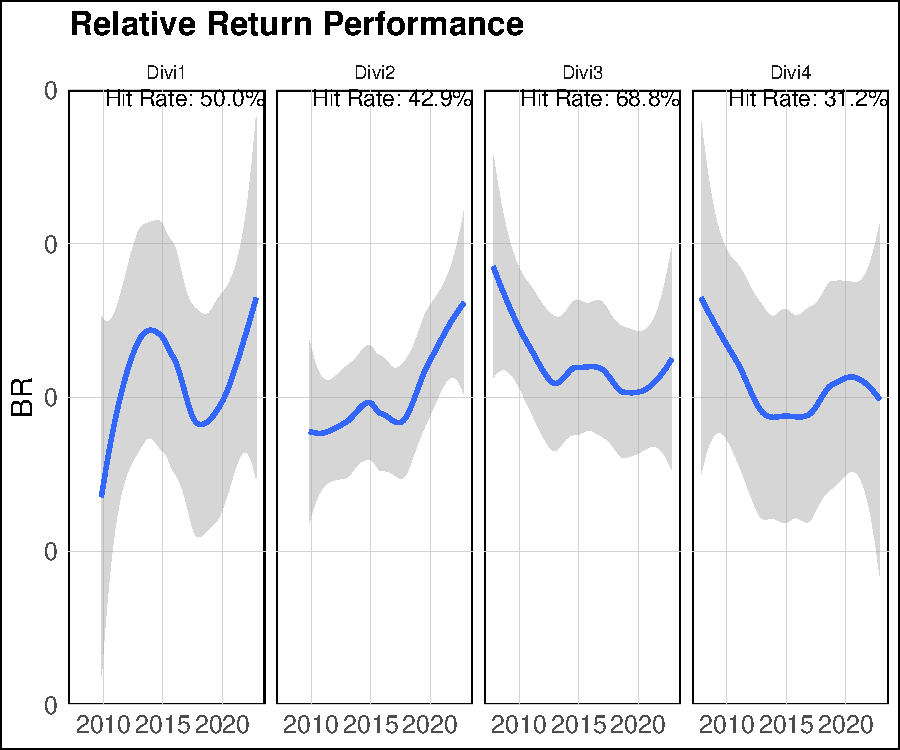
\includegraphics{Much_Ado_About_Dividends_files/figure-latex/unnamed-chunk-5-1.pdf}

\newpage

\hypertarget{conclusion}{%
\section{Conclusion}\label{conclusion}}

Over time, dividend portfolios, whether HY or DG, have exhibited
positive excess returns as indicated by cumulative returns. While the
UK\_HY index has shown the highest cumulative return, this trend is not
consistently observed across other regional indexes. Consequently, when
assessing the aggregate perspective on investor portfolio value,
dividend portfolios may not offer a reliable means to capture the value
premium consistently. However, upon stratifying these portfolios
according to different periods of market volatility, it becomes evident
that during low volatility periods, the primary determinant of
performance is not the geographical region but rather the specific
investment strategy employed. In this case, HY strategies. Surprisingly,
portfolios based in South Africa (SA) tend to perform well during these
high volatility periods, which is somewhat unconventional as such times
are typically associated with a flight to safety, and Emerging Markets
(EM) and, by extension, South Africa, are considered riskier. When
extending our analysis to encompass interest rate cycles, we observe a
contrasting effect compared to the volatility-based stratification. We
find that all strategies appear to give the highest return in hiking
cycles.

In assessing consistency, we employ the information ratio. Initially, we
discern that, at a broad level, dividend portfolios do not consistently
maintain a positive ratio over an extended investment horizon. However,
disparities in performance emerge. Notably, South African (SA) and
dividend indexes have consistently delivered positive ratios over the
past decade. In contrast, Emerging Markets (EM) and Japanese (JP)
indexes have experienced substantial declines in their information
ratios, despite seemingly consistent performance prior to 2015.
Meanwhile, the United States (US), European Union (EU), and United
Kingdom (UK) indexes have exhibited unpredictable performance over the
sampled period.

When we integrate our information ratio findings with drawdown analysis,
we observe that advanced economies have experienced the fewest drawdowns
over the sample period, with the exception of the UK. This could suggest
a relatively lower level of systematic risk in these economies.
Conversely, South African (SA) and Emerging Market (EM) drawdowns have
exhibited a declining trend, possibly indicating a reduced perception of
risk in emerging markets over time.

\newpage

\hypertarget{appendix}{%
\section{Appendix}\label{appendix}}

\hypertarget{globally-traded-dividend-portfolios-considered}{%
\subsection{Globally Traded Dividend Portfolios
Considered}\label{globally-traded-dividend-portfolios-considered}}

\begingroup\fontsize{8pt}{9pt}\selectfont
\begin{longtable}{llll}
  \toprule
TICKER & NAME & Codename & Inception Date \\ 
  \hline 
\endhead 
\hline 
{\footnotesize Continued on next page} 
\endfoot 
\endlastfoot 
 \midrule
FUDP & FTSE UK Dividend+ Index & UK\_HY &  \\ 
  M2EFDY & MSCI EM HY Gross Total Return USD Index & EM\_HY &  \\ 
  M2GBDY & MSCI UK HY Gross Total Return USD Index & UK\_HY &  \\ 
  M2JPDY & MSCI Japan HY Gross Total Return USD & JP\_HY &  \\ 
  M2USADVD & MSCI USA HY Gross Total Return USD Index & US\_HY &  \\ 
  M2WDHDVD & MSCI World HY Gross Total Return Total Return USD Index & W\_HY &  \\ 
  SPDAEET & S\&P EU 350 Dividends Aristocrats Total Return Index & EU\_DG &  \\ 
  SPJXDAJT & S\&P/JPX Dividend Aristocrats Total Return Index & JP\_DG &  \\ 
  SPDAUDT & S\&P 500 Dividend Aristocrats Total Return Index & US\_DG &  \\ 
  SPSADAZT & S\&P South Africa Dividend Aristocrats Index ZAR Gross TR & SA\_DG &  \\ 
  TJDIVD & FTSE/JSE Dividend+ Index Total Return Index & SA\_HY &  \\ 
  M2EUGDY & MSCI Europe Ex UK HYGross Total Return USD Index & EU\_HY &  \\ 
  TUKXG & FTSE 100 Total Return Index GBP & UK &  \\ 
  GDUEEGF & MSCI Daily TR Gross EM USD & EM &  \\ 
  GDDUUK & MSCI UK Gross Total Return USD Index & UK\_B &  \\ 
  TPXDDVD & Topix Total Return Index JPY & JP &  \\ 
  GDDUUS & MSCI Daily TR Gross USA USD & US &  \\ 
  GDDUWI & MSCI Daily TR Gross World USD & W &  \\ 
  SPTR350E & S\&P Europe 350 Gross Total Return Index & EU\_2 &  \\ 
  SPXT & S\&P 500 Total Return Index & JP &  \\ 
  SPXT & S\&P 500 Total Return Index & US\_2 &  \\ 
  JALSH & FTSE/JSE Africa All Share Index & SA &  \\ 
  JALSH & FTSE/JSE Africa All Share Index & SA &  \\ 
  GDDUE15X & MSCI Daily TR Gross Europe Ex UK USD & EU &  \\ 
   \bottomrule
\caption{Index Description \label{indexdes}} 
\end{longtable}
\endgroup

\hypertarget{stratified-periods-considered}{%
\subsection{Stratified Periods
Considered}\label{stratified-periods-considered}}

\newpage

\hypertarget{dividend-defintions}{%
\subsection{Dividend Defintions}\label{dividend-defintions}}

Bloomberg has two main categories for distributions: Cash Dividends and
Stock Dividends. Various kinds of distributions appear under these
definitions that do not necessarily only apply to ordinary issued shares
(the only security type that we consider in our study). In the next two
subsections we define the types of distributions that fall under these
categories and in some cases provide additional information. Our sample
only comprises of final, interim and regular cash dividends. These
dividends are categorized by Bloomberg as Normal Cash.

\hypertarget{cash-dividends}{%
\subsubsection{Cash Dividends}\label{cash-dividends}}

\begin{itemize}
\tightlist
\item
  Final: dividend declared for the financial year-end
\item
  Interim (includes 2nd interim, 3rd interim and 4th interim): dividend
  paid after a reporting period (eg. quarterly or semi-annually) Special
  Cash: dividend declared for the financial year-end or interim period
  over and above the normal dividend
\item
  Regular Cash: a dividend distribution made in cash
\item
  Omitted: A company has elected to skip a scheduled payment
\item
  Discontinued: The discontinuance of dividend payments on an ongoing
  basis
\item
  Interest on Capital: interest paid on fixed income instruments
\item
  Income: mutual fund dividends, in most cases
\item
  Liquidation: a distribution of a companies assets to shareholders
  during (interim) or after delisting (final)
\item
  Return of Capital: a non-taxable cash payment to investors from the
  company that represents a return on invested capital as opposed to a
  dividend
\item
  Memorial: a special dividend. For example a company celebrating an
  anniversary might pay a memorial dividend
\item
  Proceeds from sale of shares: a distribution of cash to shareholders
  after selling shares. For example this may occur when the company
  sells the shares of a shareholder who was not eligible to receive
  shares in an offering and then distributes the proceeds to
  shareholders
\item
  Cancelled: the cancellation of a previously declared dividend
\item
  Return Premium: special cash dividend paid from a special reserve
\item
  Preferred Rights Redemption: a company pays a dividend in exchange for
  previously issued preferred rights
\end{itemize}

\hypertarget{stock-dividends}{%
\subsection{Stock Dividends}\label{stock-dividends}}

Bonus: also known as a scrip or capitalization issue. Shareholders are
given additional stock in proportion to their holdings - Scrip: a free
issue or bonus of shares - Stock Dividend: portion of a company's
retained earnings that are distributed to shareholders in stock. The JSE
treats stock dividends as a capitalization issue \newpage

\hypertarget{references}{%
\section{References}\label{references}}

\hypertarget{refs}{}
\begin{CSLReferences}{1}{0}
\leavevmode\vadjust pre{\hypertarget{ref-al2018revisiting}{}}%
Al-Najjar, B. \& Kilincarslan, E. 2018. Revisiting firm-specific
determinants of dividend policy: Evidence from turkey. \emph{Economic
issues}. 23(1):3--34.

\leavevmode\vadjust pre{\hypertarget{ref-baker1999corporate}{}}%
Baker, H.K. \& Powell, G.E. 1999. How corporate managers view dividend
policy. \emph{Quarterly Journal of Business and Economics}. 17--35.

\leavevmode\vadjust pre{\hypertarget{ref-black1996dividend}{}}%
Black, F. 1996. The dividend puzzle. \emph{Journal of Portfolio
Management}. 8.

\leavevmode\vadjust pre{\hypertarget{ref-brzeszczynski2007dividend}{}}%
Brzeszczyński, J. \& Gajdka, J. 2007. Dividend-driven trading
strategies: Evidence from the warsaw stock exchange. \emph{International
Advances in Economic Research}. 13:285--300.

\leavevmode\vadjust pre{\hypertarget{ref-campbell2017financial}{}}%
Campbell, J.Y. 2017. \emph{Financial decisions and markets: A course in
asset pricing}. Princeton University Press.

\leavevmode\vadjust pre{\hypertarget{ref-conover2016difference}{}}%
Conover, C.M., Jensen, G.R. \& Simpson, M.W. 2016. What difference do
dividends make? \emph{Financial Analysts Journal}. 72(6):28--40.

\leavevmode\vadjust pre{\hypertarget{ref-damodaran2004investment}{}}%
Damodaran, A. 2004. \emph{Investment fables: Exposing the myths of"
can't miss" investment strategies}. FT Press.

\leavevmode\vadjust pre{\hypertarget{ref-fakir2013dividend}{}}%
Fakir, R. et al. 2013. Dividend yield as a superior investment strategy.
PhD thesis. University of Pretoria.

\leavevmode\vadjust pre{\hypertarget{ref-filbeck1997}{}}%
Filbeck, G. \& Visscher, S. 1997. Dividend yield strategies in the
british stock market. \emph{The European Journal of Finance}.
3(4):277--289.

\leavevmode\vadjust pre{\hypertarget{ref-filbeck2017dividend}{}}%
Filbeck, G., Holzhauer, H.M. \& Zhao, X. 2017. Dividend-yield
strategies: A new breed of dogs. \emph{The Journal of Investing}.
26(2):26--47.

\leavevmode\vadjust pre{\hypertarget{ref-gardner2002motley}{}}%
Gardner, D., Gardner, T. \& Maranjian, S. 2002. \emph{The motley fool
investment guide for teens: 8 steps to having more money than your
parents ever dreamed of}. Vol. 10. Simon; Schuster.

\leavevmode\vadjust pre{\hypertarget{ref-gordon1962}{}}%
Gordon, M.J. 1962. The savings investment and valuation of a
corporation. \emph{The Review of Economics and Statistics}. 37--51.

\leavevmode\vadjust pre{\hypertarget{ref-lemmon2015dividend}{}}%
Lemmon, M.L. \& Nguyen, T. 2015. Dividend yields and stock returns in
hong kong. \emph{Managerial Finance}. 41(2):164--181.

\leavevmode\vadjust pre{\hypertarget{ref-miller}{}}%
Miller, M.H. \& Modigliani, F. 1961. Dividend policy, growth, and the
valuation of shares. \emph{The Journal of Business}. 34(4):411--433.

\leavevmode\vadjust pre{\hypertarget{ref-miller1985dividend}{}}%
Miller, M.H. \& Rock, K. 1985. Dividend policy under asymmetric
information. \emph{The Journal of finance}. 40(4):1031--1051.

\leavevmode\vadjust pre{\hypertarget{ref-o1991beating}{}}%
O'higgins, M. \& Downes, J. 1991. \emph{(No Title)}.

\leavevmode\vadjust pre{\hypertarget{ref-suwanna2012impacts}{}}%
Suwanna, T. 2012. Impacts of dividend announcement on stock return.
\emph{Procedia-Social and Behavioral Sciences}. 40:721--725.

\leavevmode\vadjust pre{\hypertarget{ref-van2013advanced}{}}%
Van Deventer, D.R., Imai, K. \& Mesler, M. 2013. \emph{Advanced
financial risk management: Tools and techniques for integrated credit
risk and interest rate risk management}. John Wiley \& Sons.

\leavevmode\vadjust pre{\hypertarget{ref-visscher2003dividend}{}}%
Visscher, S. \& Filbeck, G. 2003. Dividend-yield strategies in the
canadian stock market. \emph{Financial Analysts Journal}. 59(1):99--106.

\leavevmode\vadjust pre{\hypertarget{ref-wang2011dogs}{}}%
Wang, C., Larsen, J.E., Ainina, M.F., Akhbari, M.L. \& Gressis, N. 2011.
The dogs of the dow in china. \emph{International Journal of Business
and Social Science}. 2(18).

\end{CSLReferences}

\bibliography{Tex/ref}





\end{document}
